\documentclass{beamer}
\usetheme{sidebar}
\usecolortheme{rose}

\begin{document}
\title{Universidad Veracruzana}  
\subtitle{Centro de Investigaciones Cerebrales\\Computación Científica y Bioinformática\\
"Resultados del Acoplamiento Molecular tipo Doking"}
\author{Psic. Lázaro Salomón Lara}
\date{} 
\begin{frame}
\titlepage
Profesores: Dr. Gonzalo Aranda Abreu, Dr. Adolfo Centeno
\end{frame}


\begin{frame}\frametitle{Acoplamiento Molecular}
El acoplamiento molecular automatizado tiene como objetivo proponer un modelo de unión entre dos moléculas. Este método ha sido útil en química farmacéutica y en el descubrimiento de nuevos fármacos por medio del entendimiento de las fuerzas de interacción involucradas en el reconocimiento molecular.
 \begin{figure}[h]
      \centering
      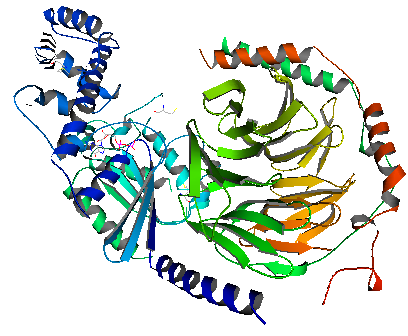
\includegraphics[scale=2]{docking.png}

      \label{fig:my_label}
  \end{figure}  
\end{frame} 


\begin{frame}\frametitle{Metodología}
Se hizo uso del software "AutoDockTools" para modelar el Acoplamiento Molecular entre la Proteína S de superficie (Spike Protein) del virus SARS-Cov2 y el fármaco Amantadina
 \begin{figure}[h]
      \centering
      
\includegraphics[scale=0.6]{autodock.png}

      \label{fig:my_label}
  \end{figure}  
\end{frame} 


\begin{frame}\frametitle{Implementación}
El procedimiento se realizó tal cual se presenta descrito en el manual "Using AutoDock 4 and
AutoDock Vina with AutoDockTools: A Tutorial" de Ruth Huey, Garrett M. Morris y Stefano Forli, del Scripps Research Institute
Molecular Graphics Laboratory
\end{frame} 


\begin{frame}\frametitle{Implementación}
Se inició instalando y abriendo el software
  \begin{figure}[h]
      \centering
      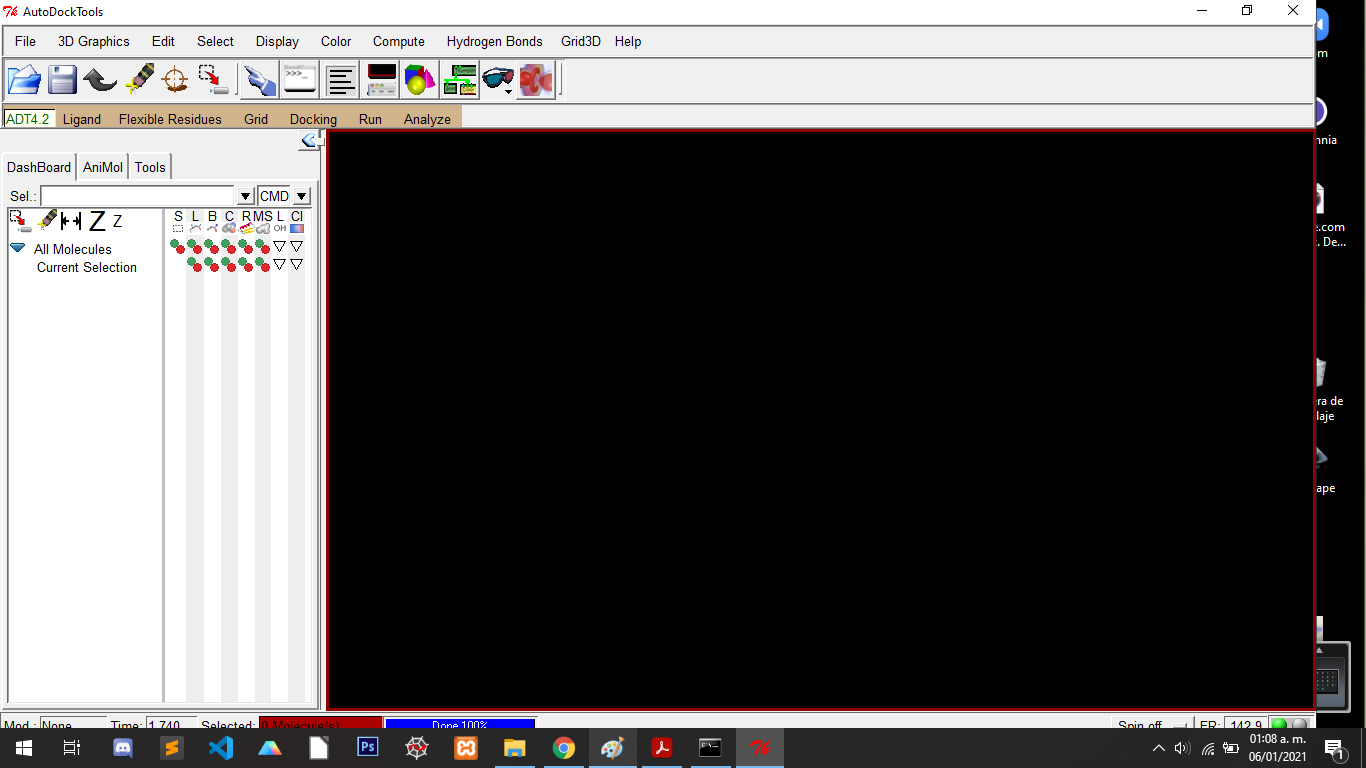
\includegraphics[scale=0.25]{soft.png}
      \caption{AutoDockTools}
      \label{fig:my_label}
  \end{figure}  
\end{frame} 


\begin{frame}\frametitle{Implementación}
Se cargó la Proteína S del SARS-Cov2 (7ddd.pdb) con formato Protein Data Bank)
  \begin{figure}[h]
      \centering
      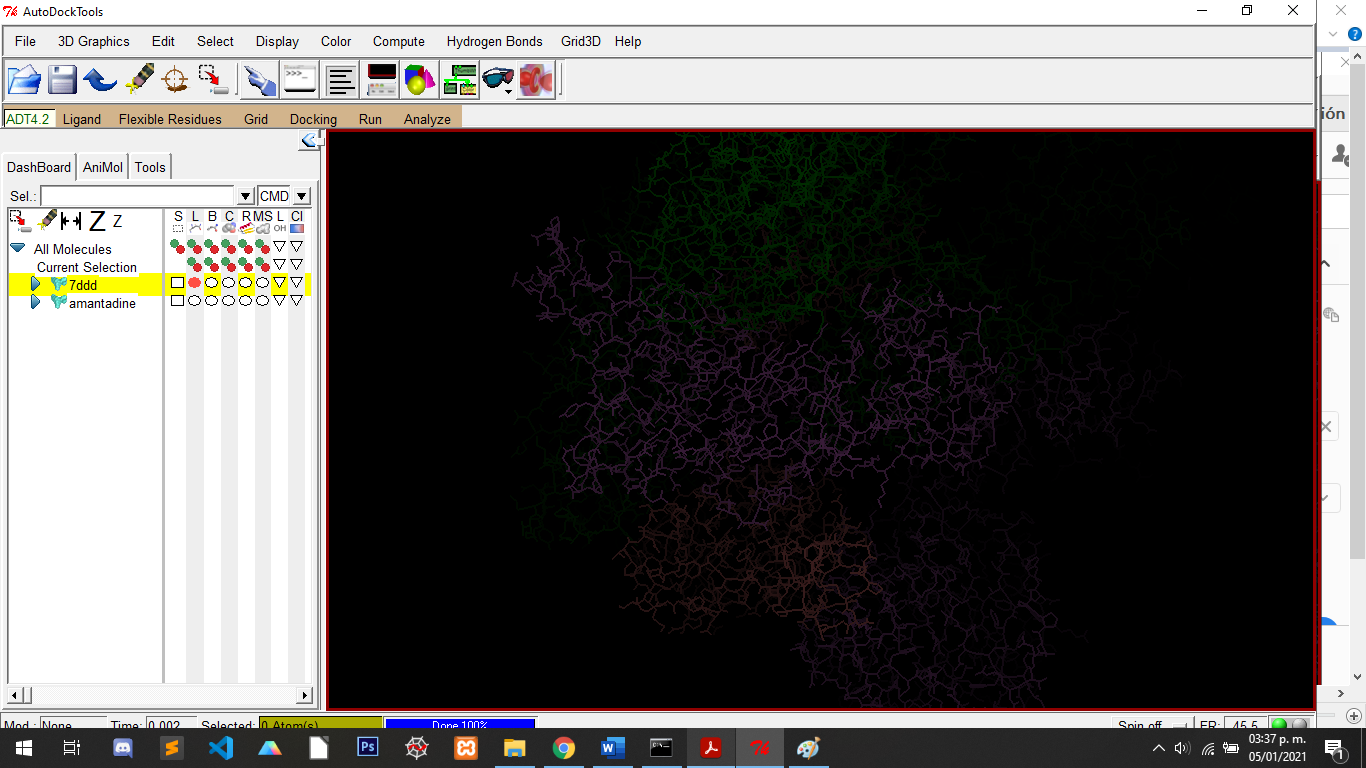
\includegraphics[scale=0.25]{S.png}
      \caption{Proteína S}
      \label{fig:my_label}
  \end{figure}  
\end{frame} 


\begin{frame}\frametitle{Implementación}
Se cargó el ligando Amantadina (amantadine.pdb) con formato Protein Data Bank)
  \begin{figure}[h]
      \centering
      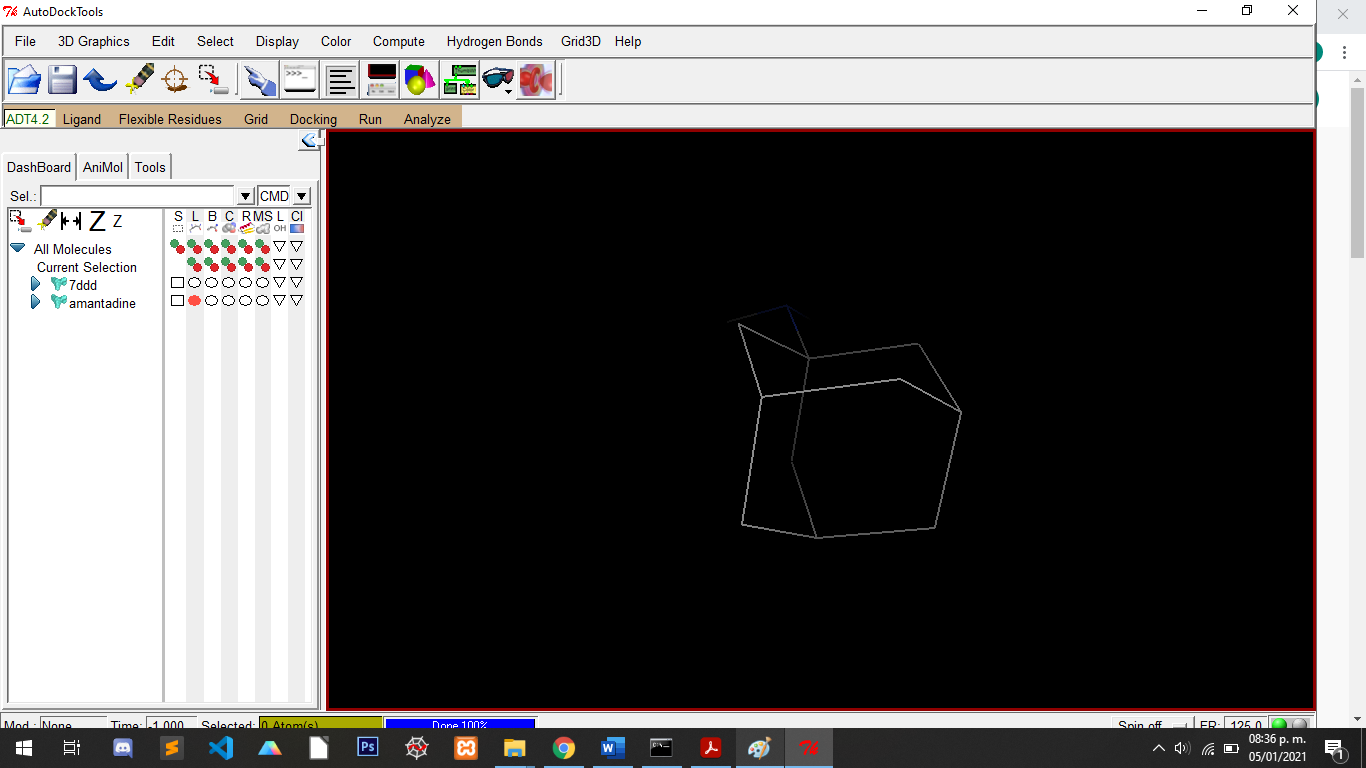
\includegraphics[scale=0.25]{Ligando.png}
      \caption{Amantadina}
      \label{fig:my_label}
  \end{figure}  
\end{frame} 


\begin{frame}\frametitle{Implementación}
Se prepara el receptor, eliminando el solvatado, agregandole los hidrógenos y configurándolo como macromolécula y guardándolo en formato *.pdbqt
  \begin{figure}[h]
      \centering
      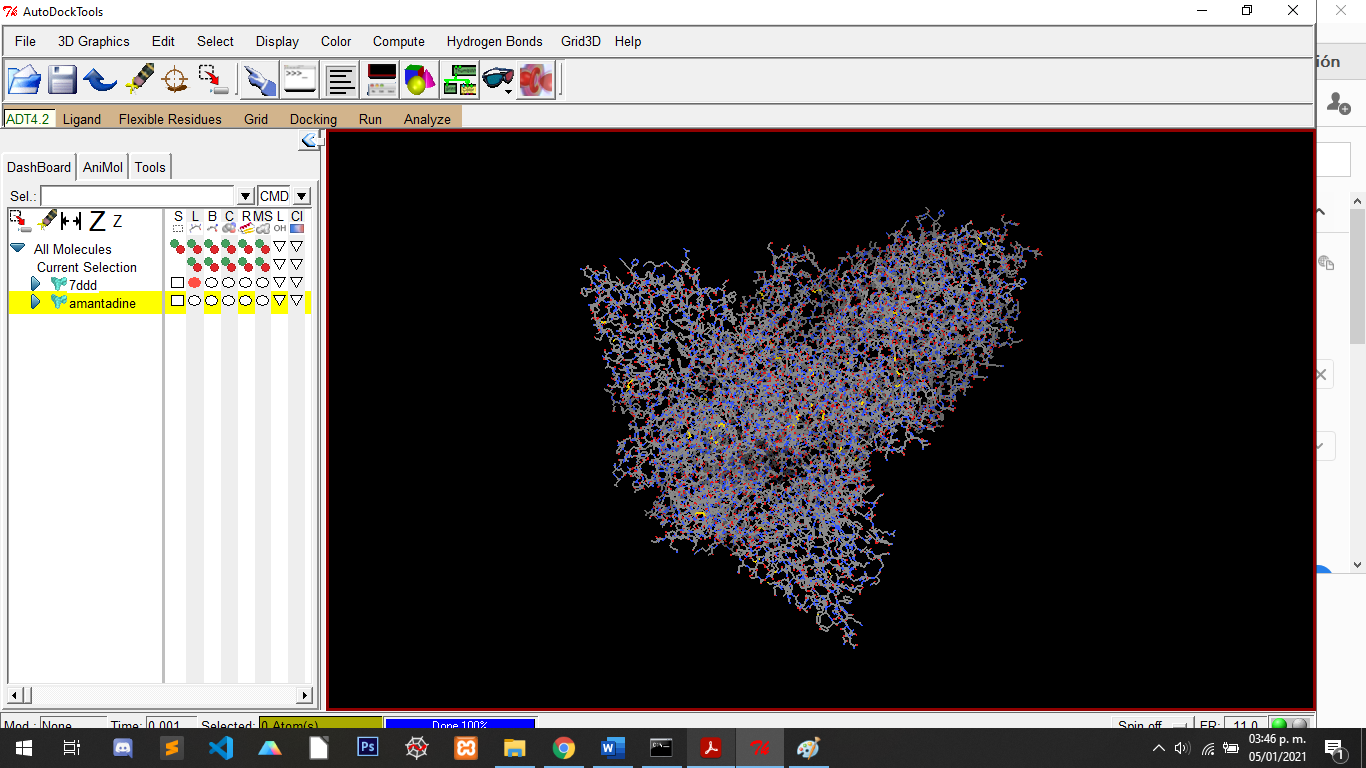
\includegraphics[scale=0.25]{Receptor.png}
      \caption{Preparando el Receptor}
      \label{fig:my_label}
  \end{figure}  
\end{frame} 


\begin{frame}\frametitle{Implementación}
Se prepara el receptor definiendo el Grid Box como espacio de búsqueda, esto es, su tamaño y coordenadas
  \begin{figure}[h]
      \centering
      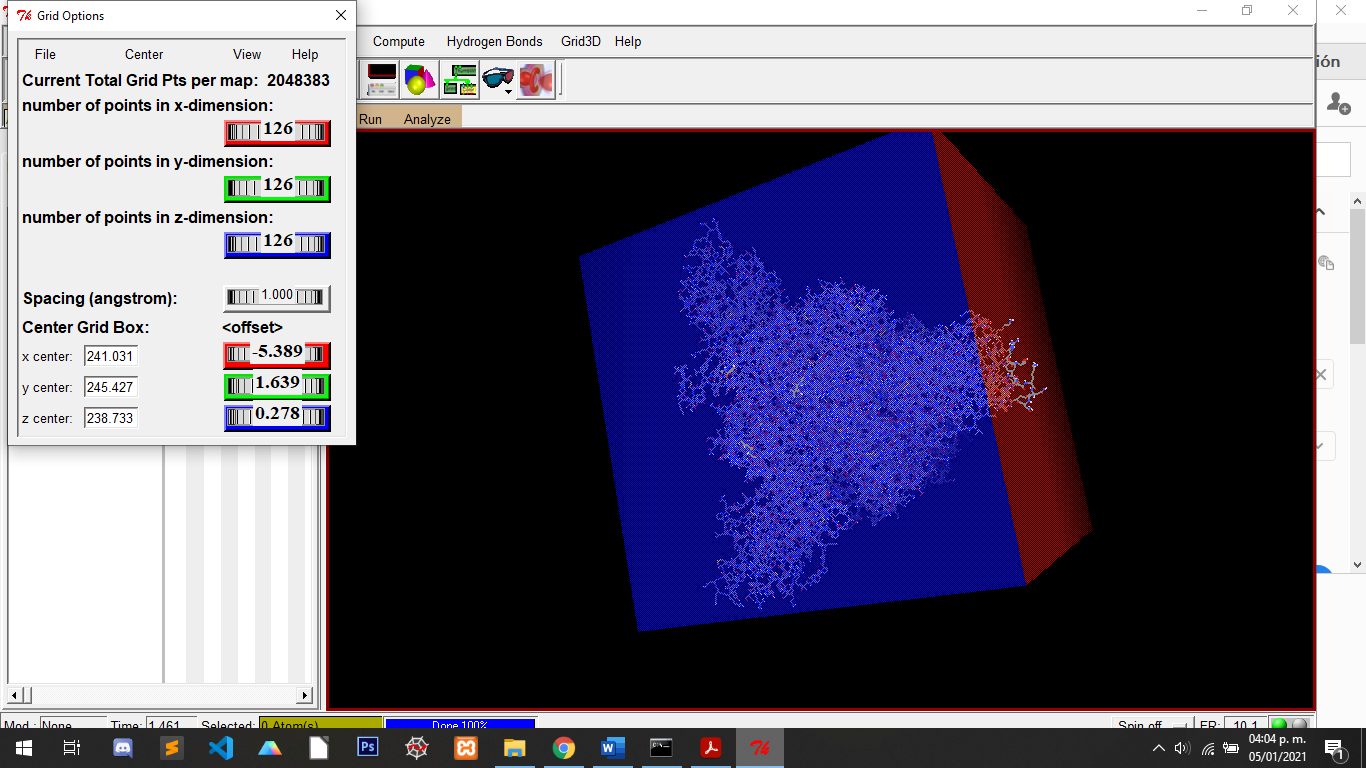
\includegraphics[scale=0.25]{Busqueda.png}
      \caption{Preparando el Espacio de Búsqueda}
      \label{fig:my_label}
  \end{figure}  
\end{frame} 


\begin{frame}\frametitle{Implementación}
Se prepara el ligando, encontrando el eje de torsión, configurando el número de torsiones, definiéndolo como ligando principal de la macromolécula y guardándolo en formato *.pdbqt
  \begin{figure}[h]
      \centering
      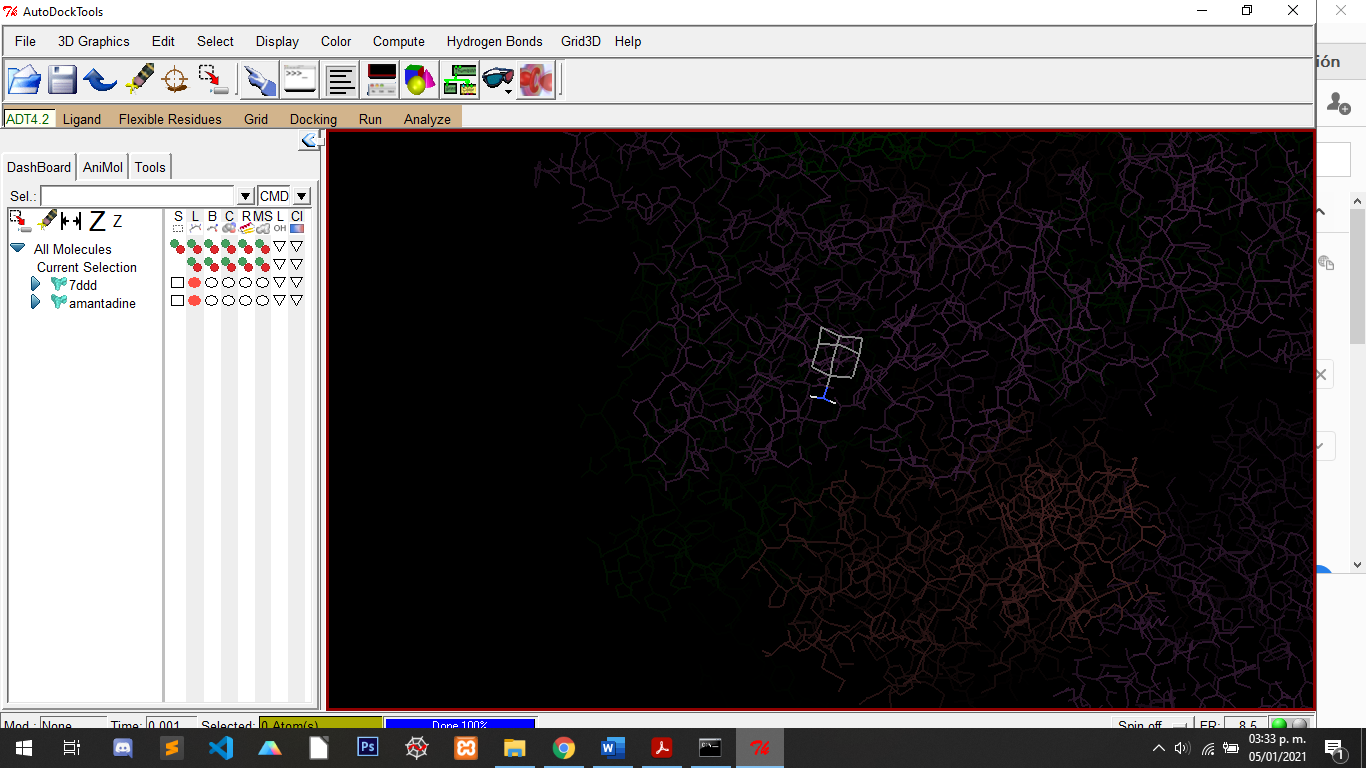
\includegraphics[scale=0.25]{Lig.png}
      \caption{Preparando el Ligando}
      \label{fig:my_label}
  \end{figure}  
\end{frame} 


\begin{frame}\frametitle{Implementación}
Se genera archivo de texto de configuración con las coordenadas del Grid Box
  \begin{figure}[h]
      \centering
      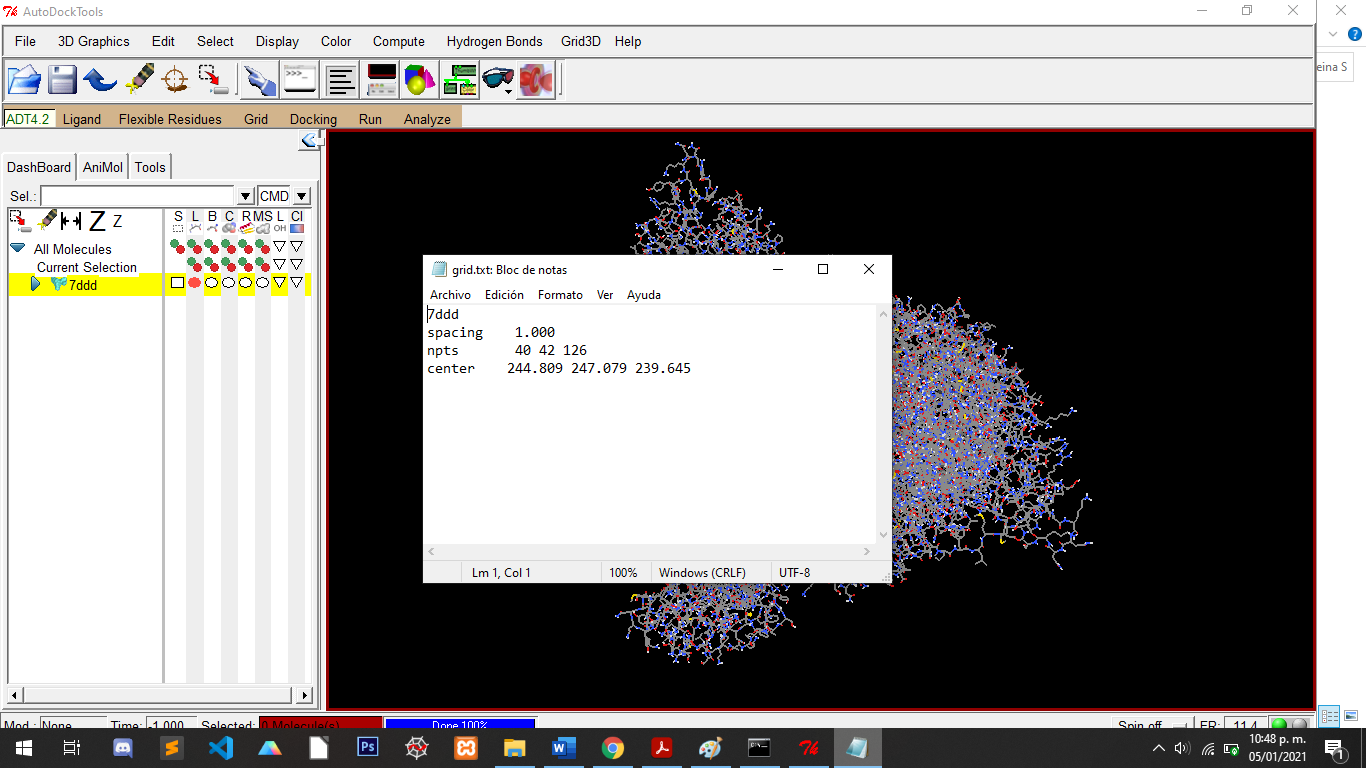
\includegraphics[scale=0.25]{Grid.png}
      \caption{Archivo de configuración del Grid Box}
      \label{fig:my_label}
  \end{figure}  
\end{frame} 


\begin{frame}\frametitle{Implementación}
Se genera archivo de texto de configuración con el nombre de los archivos del receptor y el ligando
  \begin{figure}[h]
      \centering
      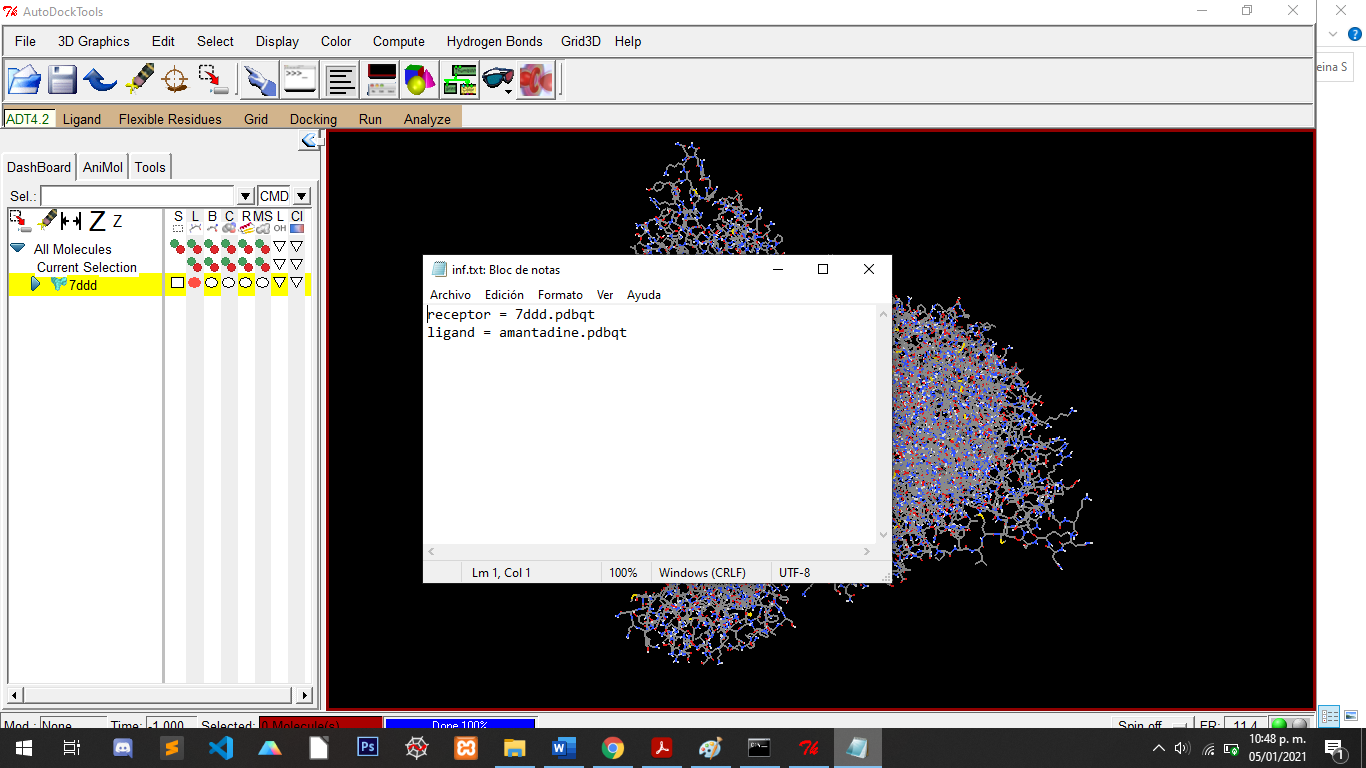
\includegraphics[scale=0.25]{Inf.png}
      \caption{Receptor y Ligando}
      \label{fig:my_label}
  \end{figure}  
\end{frame} 


\begin{frame}\frametitle{Implementación}
Intentando correr el Acoplamiento
  \begin{figure}[h]
      \centering
      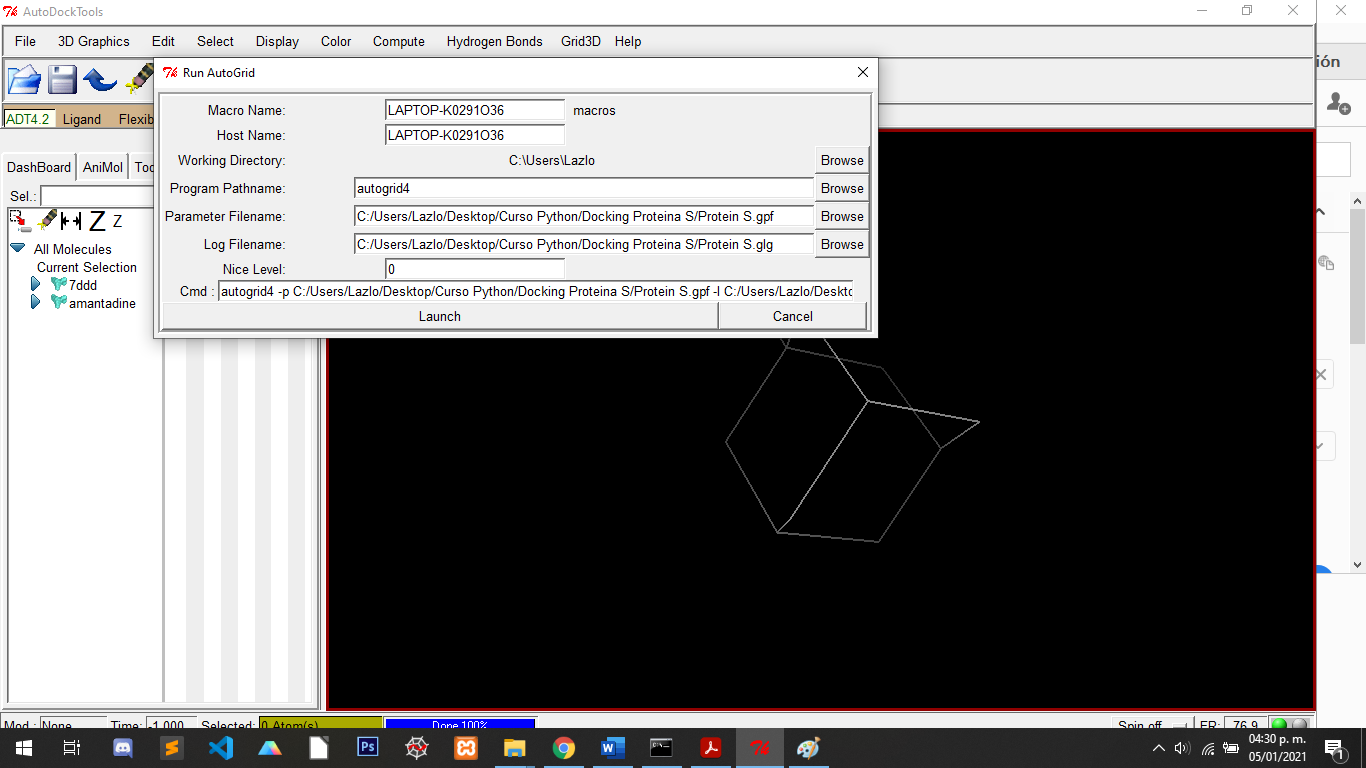
\includegraphics[scale=0.25]{run.png}
      \caption{Corriendo el Acoplamiento Molecular}
      \label{fig:my_label}
  \end{figure}  
\end{frame} 


\begin{frame}\frametitle{Implementación}
Error presentado. Se intentó de diversas maneras corregirlo, pero resultó imposible
  \begin{figure}[h]
      \centering
      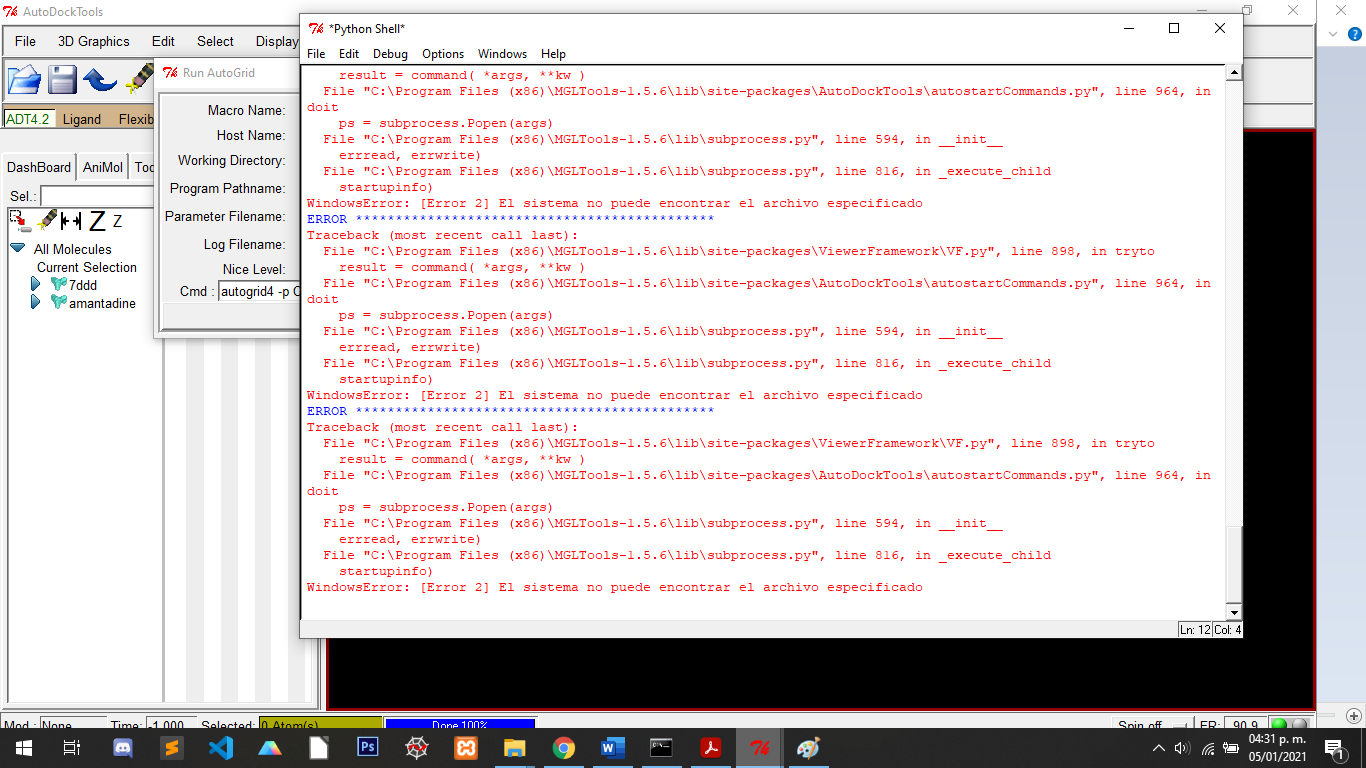
\includegraphics[scale=0.25]{Error.png}
      \caption{Error en el Acoplamiento Molecular}
      \label{fig:my_label}
  \end{figure}  
\end{frame}










\end{document}